\documentclass[border=10pt]{standalone}

\usepackage{tikz}
\usepackage{tikzsymbols}
\usetikzlibrary{calc,patterns,shapes.geometric}

\def\centerarc[#1](#2)(#3:#4:#5){\draw[#1] ($(#2)+({#5*cos(#3)},{#5*sin(#3)})$) arc (#3:#4:#5);}

\begin{document}
	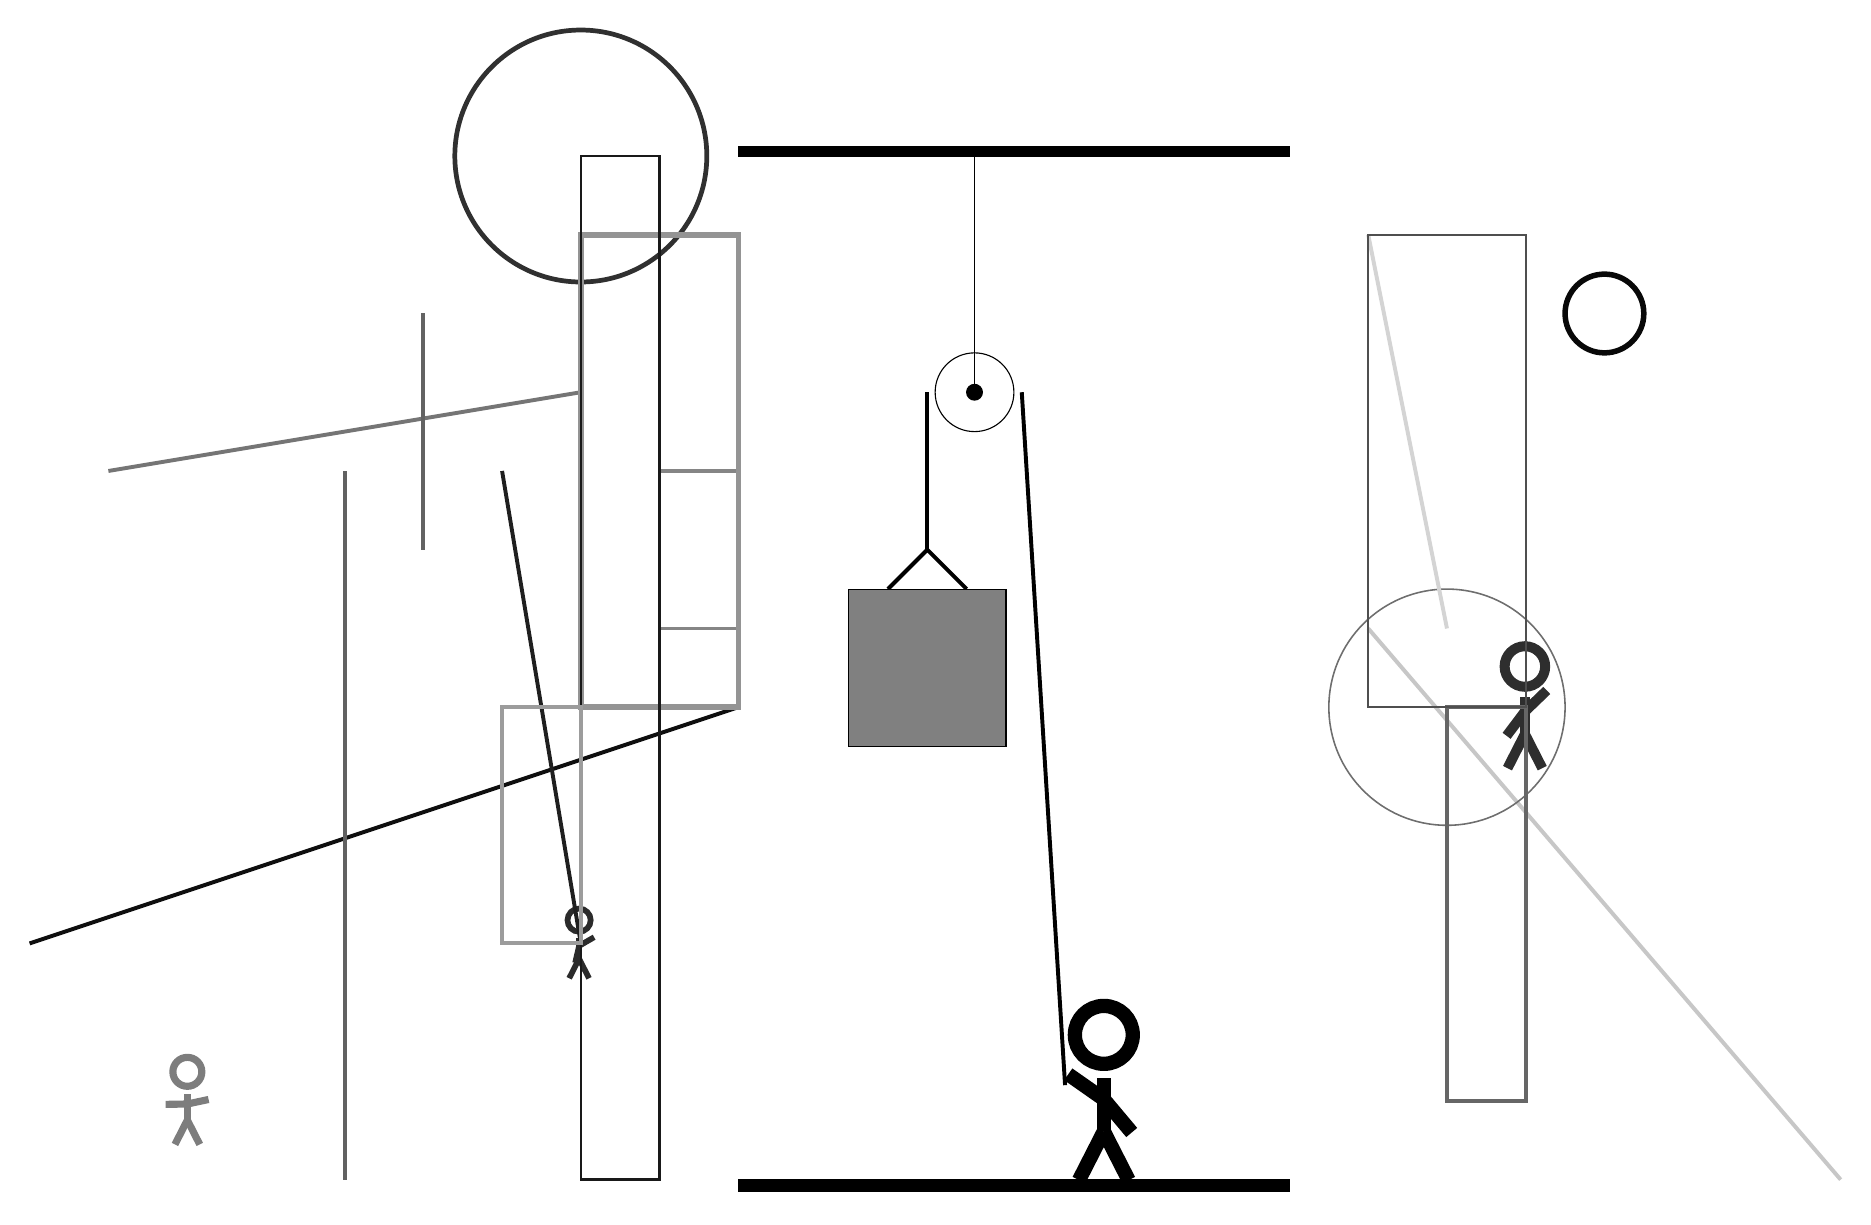
\begin{tikzpicture}
		%%%%% START %%%%%
		
		\draw[fill=black] (-2, 10) rectangle (5, 10.125);
		
		\draw (1, 7) circle (0.5);
		\draw[fill=black] (1, 7) circle (0.1);
		\draw (1, 10) -- (1, 7);
		
		\draw[line width=0.5mm] (-0.1, 4.5) -- (0.4, 5.0) -- (0.9, 4.5);
		\draw[fill=black!50] (-0.6, 4.5) rectangle (1.4, 2.5);
		
		\draw[line width=0.5mm] (0.4, 7) -- (0.4, 5.0);
		\centerarc[line width=0.5mm](1, 7)(0:180:0.6);
		\draw[line width=0.5mm](1.6, 7) -- (2.15, -1.8);
		
		\node at (2.6, -1.9) {\Strichmaxerl[10][-35][-50]};
		
		\node[line width=0.3mm, color=black!83] at (-4, 0) {\Strichmaxerl[4][77][30]};
		
		\draw[line width=0.5mm, color=black!22](6, 4) -- (12, -3);
		\draw[line width=0.4mm, color=black!48] (-2, 4) rectangle (-3, 6);
		\draw[line width=0.5mm, color=black!54](-4, 7) -- (-10, 6);
		\node[line width=0.7mm, color=black!51] at (-9, -2) {\Strichmaxerl[5][1][12]};
		\draw [line width=0.6mm, color=black!81](-4, 10) circle (1.6);
		\draw[line width=0.5mm, color=black!94](-2, 3) -- (-11, 0);
		\draw [line width=0.2mm, color=black!57](7, 3) circle (1.5);
		\node[line width=0.3mm, color=black!82] at (8, 3) {\Strichmaxerl[7][53][44]};
		
		\draw[line width=0.5mm, color=black!61](-6, 8) -- (-6, 5);
		\draw[line width=0.5mm, color=black!60] (7, -2) rectangle (8, 3);
		\draw[line width=0.7mm, color=black!42] (-4, 9) rectangle (-2, 3);
		\draw[line width=0.5mm, color=black!88](-5, 6) -- (-4, 0);
		
		\draw[line width=0.5mm, color=black!17](6, 9) -- (7, 4);
		\draw[line width=0.3mm, color=black!90] (-3, 10) rectangle (-4, -3);
		\draw [line width=0.7mm, color=black!97](9, 8) circle (0.5);
		\draw[line width=0.3mm, color=black!69] (6, 9) rectangle (8, 3);
		\draw[line width=0.5mm, color=black!39] (-4, 0) rectangle (-5, 3);
		\draw[line width=0.5mm, color=black!62](-7, -3) -- (-7, 6);
		
		
		\draw[fill=black] (-2, -3) rectangle (5, -3.15);
		
		%%%%% END %%%%%
	\end{tikzpicture}
\end{document}